\documentclass[letterpaper,10pt]{book}
% Change to 10 pt
\usepackage{pdfpages}
\usepackage{morewrites}			% to counteract the no write space problem
\setcounter{tocdepth}{6}

\usepackage[framemethod=TikZ]{mdframed}

\usepackage{fancyhdr}

\usepackage{paralist}
\usepackage{amsmath}
\usepackage{amsfonts}
\usepackage{amssymb}
\usepackage{graphicx}

\usepackage{datetime}
%\usepackage{ulem}

%\usepackage[nottoc]{toobibind}

\usepackage[inline]{enumitem}

% Outer margin at 2.50 is exacty correct to fit the ``corruption alert'' tables
\usepackage[inner=1.0in, outer=2.50in, top=2.54cm,bottom=2.54cm, marginparwidth=2.25in]{geometry}

\usepackage{marginnote}
\usepackage{longtable}
\usepackage{booktabs}
\usepackage{xcolor}

\usepackage{soul}

%%%%%%%%%%%%
\definecolor{ForestGreen}{rgb}{0.00,0.29,0.098}
%%%%%%%%%%%%

\usepackage{marginnote}

\usepackage{imakeidx} 
\usepackage[
	backref=true,
	style=numeric,
%	citestyle=numeric,
	backend=bibtex
	]{biblatex}
\usepackage[driverfallback=hypertex,colorlinks=True]{hyperref}
\usepackage{cleveref}

\makeindex[name=scripture,columnsep=20pt, columnseprule=True,columns=3, title=Scripture References]
\makeindex[name=speaker,columnsep=20pt, columnseprule=True,,columns=2, title=Sermon Creator]
\makeindex[name=series,columnsep=20pt, columnseprule=True,,columns=2, title=Sermon Series]
\makeindex[name=date,columnsep=20pt, columnseprule=True,columns=2, title=Sermon Date]

\makeindex[name=event,columnsep=20pt, columnseprule=True,columns=2, title=Event]

\makeindex[name=topic,columnsep=20pt, columnseprule=True,columns=2, title=Topic]
\makeindex[name=AWIP,columnsep=20pt, columnseprule=True,columns=3, title=All Words in Passage]
\makeindex[name=NWIV,columnsep=20pt, columnseprule=True,columns=3, title=Number of Words in Verse]
\makeindex[name=PNIP,columnsep=20pt, columnseprule=True,columns=3, title=Proper Names in Passage]
\makeindex[name=PEIP,columnsep=20pt, columnseprule=True,columns=2, title=Prophetic Events in Passage]

\makeindex[name=TWPAQ,columnsep=20pt, columnseprule=True,columns=1, title=13-Word Phrases and Quotes]
\makeindex[name=PFTTIS,columnsep=20pt, columnseprule=False,columns=3, title=Phrases found 13 times in scripture]
\makeindex[name=WFTTIS,columnsep=20pt, columnseprule=False,columns=3, title=Words found 13 times in scripture]
\makeindex[name=WFITV,columnsep=20pt, columnseprule=False,columns=3, title=Words found in exactly 13 verses]
\makeindex[name=EVENTS,columnsep=20pt, columnseprule=False,columns=2, title=Sermon Log by Place]
\makeindex[name=QUESTIONS,columnsep=20pt, columnseprule=False,columns=2, title=Bible Questions]

\makeindex[name=DOCTRINES,columnsep=20pt, columnseprule=False,columns=2, title=Doctrines]

\makeindex[name=SONGS,columnsep=20pt, columnseprule=False,columns=1, title=Songs]
\makeindex[name=LOCATION,columnsep=20pt, columnseprule=False,columns= 2, title=Location]
\makeindex[name=FACEBOOK,columnsep=20pt, columnseprule=False,columns=2, title=Facebook]

%%%%%%%%%%%%%%%%% EXTRA COLORS
\definecolor{champagne}{rgb}{0.97,0.91,0.81}
\definecolor{bone}{rgb}{0.89,0.85,0.79}


\pagestyle{fancy}
\fancyhf{}
\fancyhead[LE,RO]{\today}
\fancyhead[RE,LO]{Daily Bible Reading}
\fancyhead[CE,CO]{-page \thepage  - }

\fancyfoot[CO,CE]{\leftmark}
%\fancyfoot[LE,RO]{CSCE 692, HW1}

\title{DBR\\
Daily \\ Reads}
\author{Keith Anthony \\
\today }
%\title

%+/ffffff +   \pagenumbering{gobble}

\bibliography{Bibliographies/All20220108}

%%%%% TWEAKS:
%%% - distance from fcolorbox frame to text
\setlength{\fboxsep}{1.0pt}

\usepackage[utf8]{inputenc}
\usepackage{tikz}

%%%%%%%%%%%%%%%%%%%%%%%%%%%%%%%%%%%%%%%%%%%%%%%%%%%%%%%%%%%%%%%%%%%%%%%%%%%%%%%%
%%%%%%%%%%%%%%%%%%%%%%%%%%%%%%%%%%%%%%%%%%%%%%%%%%%%%%%%%%%%%%%%%%%%%%%%%%%%%%%%
%%%%%%%%%%%%%%%%%%%%%%%%%%%%%%%%%%%%%%%%%%%%%%%%%%%%%%%%%%%%%%%%%%%%%%%%%%%%%%%%
%%%%%%%%%%%%%%%%%%%%%%%%%%%%%%%%%%%%%%%%%%%%%%%%%%%%%%%%%%%%%%%%%%%%%%%%%%%%%%%%
%%%%%%%%%%%%%%%%%%%%%%%%%%%%%%%%%%%%%%%%%%%%%%%%%%%%%%%%%%%%%%%%%%%%%%%%%%%%%%%%



\begin{document}

%%%%%%%%%%%%
%%%%%%%%%%%% Tile Page
%%%%%%%%%%%%
\begin{titlepage}

\begin{flushright}
\rightskip=-2.5cm
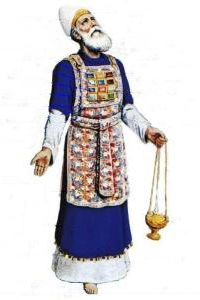
\includegraphics[width=50mm,scale=1.5]{Extras/Melchisedec.jpg}
\vspace{0.4in}  % Create a title for the document and write it in bold font
\LARGE{\textbf{\date}} % Again, do a line break
\linebreak 
% Create a subtitle \large{with Outlines, Statistics, Cross References, and Notes}
\vspace{0.5in}
\begin{flushleft}
\LARGE{Day \#30: Sunday, 30 January 2022 PLAIN  \\}\vspace{0.25in}
\LARGE{Exodus 37-38 Psalm 30 Proverb 30}
\end{flushleft}
\vspace{0.6in}
\bigskip

\normalsize{Xenia, Oh.\\}
\normalsize{created: \today}
\vspace{1.3in}

\end{flushright}
\end{titlepage}

%%%%%%%%%%%%
%%%%%%%%%%%%
%%%%%%%%%%%%

%\titleJE

\newpage 

\tableofcontents\hypertarget{TOC}{}
\listoffigures
\listoftables

\hyphenation{A-bim-e-lech bre-thren E-phra-im  Gib-e-o-nites Jer-u-sa-lem through-out Phil-i-stines The-o-phil-us Am-a-le-kites ven-geance Mesh-el-e-mi-ah onan-ism Phar-a-oh thoughts grev-ous-ness Hach-a-liah adul-ter-er Shad-rach}

%\fcolorbox{black}{bone}{TEXT}
%%%%%%%%%%%%%%%%% EXTRA COLORS
%%%%%%%%%%%%%%%%% EXTRA COLORS
%%%%%%%%%%%%%%%%% EXTRA COLORS
\definecolor{champagne}{rgb}{0.97,0.91,0.81}
\definecolor{bone}{rgb}{0.89,0.85,0.79}

\definecolor{ForestGreen}{rgb}{0.00,0.29,0.098}
\definecolor{GIVING}{cmyk}{1,0.0,0.72,.1}

\definecolor{MLPE}{cmyk}{1,1,0,.45}
\definecolor{SOCCER}{cmyk}{.77, 0, .42, .49}
\definecolor{PAYBILL}{cmyk}{0,0.83,0.76,0.07}
\definecolor{SERMON}{cmyk}{.14,.9,0,.30} % aka seance \href{http://www.flatuicolorpicker.com/purple-cmyk-color-model/}{seance}
\definecolor{BIBLE}{cmyk}{0,.17,.74,.17}
\definecolor{WORKBLUE}{cmyk}{1, .5, 0, .6}
\definecolor{myOrange}{cmyk}{0, .4, .98, .03}
\definecolor{myTan}{cmyk}{0.0,.07,.17,.10}
\definecolor{myRed}{cmyk}{0,1,1,0}
\definecolor{myWhite}{cmyk}{0,0,0,0}
\definecolor{BLUESoD}{cmyk}{.97,.84,0,.04}
\definecolor{WHITE}{cmyk}{0,0,0,0}
\definecolor{OLDGOLD}{cmyk}{0.05,0.3,1.00,0}
\definecolor{CASTLETON}{cmyk}{1,0,0.31,0.66}
\definecolor{cadmiumgreen}{rgb}{0.0, 0.42, 0.24}
\definecolor{jungle}{rgb}{0.203,0.4882,0.1718}
\definecolor{MYGOLD}{rgb}{1,.84,0}

\definecolor{MYLIGHTGRAY}{rgb}{.85,.85,.85}

\definecolor{codegreen}{rgb}{0,0.6,0}
\definecolor{codegray}{rgb}{0.5,0.5,0.5}
\definecolor{codepurple}{rgb}{0.58,0,0.82}
\definecolor{backcolour}{rgb}{0.95,0.95,0.92}



\mdfdefinestyle{MyFrame}{%
    linecolor=blue,
    outerlinewidth=2pt,
    roundcorner=5pt,
    innertopmargin=\baselineskip,
    innerbottommargin=\baselineskip,
    innerrightmargin=10pt,
    innerleftmargin=10pt,
    backgroundcolor=gray!25!white}


\mdfdefinestyle{MyFrame2}{%
    linecolor=black,
    outerlinewidth=2pt,
    roundcorner=5pt,
    innertopmargin=\baselineskip,
    innerbottommargin=\baselineskip,
    innerrightmargin=10pt,
    innerleftmargin=10pt,
    backgroundcolor=yellow!25!white}



%%%%%
%% for PFTTIS list
%%%%%

%%% And Joseph said unto
\index[PFTTIS]{And Joseph said unto!Genesis!Gen 40:008}
\index[PFTTIS]{And Joseph said unto!Genesis!Gen 40:012}
\index[PFTTIS]{And Joseph said unto!Genesis!Gen 41:025}
\index[PFTTIS]{And Joseph said unto!Genesis!Gen 42:014}
\index[PFTTIS]{And Joseph said unto!Genesis!Gen 42:018}
\index[PFTTIS]{And Joseph said unto!Genesis!Gen 44:015}
\index[PFTTIS]{And Joseph said unto!Genesis!Gen 45:003}
\index[PFTTIS]{And Joseph said unto!Genesis!Gen 45:004}
\index[PFTTIS]{And Joseph said unto!Genesis!Gen 46:031}
\index[PFTTIS]{And Joseph said unto!Genesis!Gen 48:009}
\index[PFTTIS]{And Joseph said unto!Genesis!Gen 48:018}
\index[PFTTIS]{And Joseph said unto!Genesis!Gen 50:019}
\index[PFTTIS]{And Joseph said unto!Genesis!Gen 50:024}


%%% a shadow
\index[PFTTIS]{a shadow!1Chronicles!1Chr 029:15}
\index[PFTTIS]{a shadow!Job!Job 008:09}
\index[PFTTIS]{a shadow!Job!Job 014:02}
\index[PFTTIS]{a shadow!Job!Job 017:07}
\index[PFTTIS]{a shadow!Psalm!Psa 102:011}
\index[PFTTIS]{a shadow!Psalm!Psa 144:004}
\index[PFTTIS]{a shadow!Ecclesiastes!Eccl 006:012}
\index[PFTTIS]{a shadow!Ecclesiastes!Eccl 008:013}
\index[PFTTIS]{a shadow!Isaiah!Isa 04:006}
\index[PFTTIS]{a shadow!Isaiah!Isa 25:004}
\index[PFTTIS]{a shadow!Jonah!Jnh 04:06}
\index[PFTTIS]{a shadow!Colossians!Col 02:017}
\index[PFTTIS]{a shadow!Hebews!Heb 10:001}

%%% blessed is the man
\index[PFTTIS]{blessed is the man!Psalm!Psa 001:001}
\index[PFTTIS]{blessed is the man!Psalm!Psa 032:002}
\index[PFTTIS]{blessed is the man!Psalm!Psa 034:008}
\index[PFTTIS]{blessed is the man!Psalm!Psa 065:004}
\index[PFTTIS]{blessed is the man!Psalm!Psa 084:005}
\index[PFTTIS]{blessed is the man!Psalm!Psa 084:012}
\index[PFTTIS]{blessed is the man!Psalm!Psa 094:012}
\index[PFTTIS]{blessed is the man!Psalm!Psa 112:001}
\index[PFTTIS]{blessed is the man!Proverbs!Pro 008:034}
\index[PFTTIS]{blessed is the man!Isaiah!Isa 056:002}
\index[PFTTIS]{blessed is the man!Jeremiah!Jer 017:007}
\index[PFTTIS]{blessed is the man!Romans!Rom 004:008}
\index[PFTTIS]{blessed is the man!James!Jam 001:012}


%%% carry them
\index[PFTTIS]{carry them!Leviticus!Lev 14:045}
\index[PFTTIS]{carry them!Numbers!Num 11:012}
\index[PFTTIS]{carry them!Joshua!Jsh 04:003}
\index[PFTTIS]{carry them!1Samuel!1Sam 20:040}
\index[PFTTIS]{carry them!1Kings!1Kng 08:046}
\index[PFTTIS]{carry them!2Chronicles!2Chr 06:036}
\index[PFTTIS]{carry them!Ezra!Ezra 05:015}
\index[PFTTIS]{carry them!Isaiah!Isa 40:011}
\index[PFTTIS]{carry them!Isaiah!Isa 41:016}
\index[PFTTIS]{carry them!Isaiah!Isa 57:013}
\index[PFTTIS]{carry them!Jeremiah!Jer 20:004}
\index[PFTTIS]{carry them!Jeremiah!Jer 20:005}
\index[PFTTIS]{carry them!Jeremiah!Jer 43:012}


\index[PFTTIS]{good tidings!2Samuel!2Sam 18:027}
\index[PFTTIS]{good tidings!1Kings!1Ki 01:042}
\index[PFTTIS]{good tidings!2Kings!2Ki 07:009 (2x)}
\index[PFTTIS]{good tidings!Isaiah!Isa 40:009 (2x)}
\index[PFTTIS]{good tidings!Isaiah!Isa 41:007}
\index[PFTTIS]{good tidings!Isaiah!Isa 52:007}
\index[PFTTIS]{good tidings!Isaiah!Isa 61:001}
\index[PFTTIS]{good tidings!Nahum!Nah 01:005}
\index[PFTTIS]{good tidings!Luke!Lk 02:010}
\index[PFTTIS]{good tidings!1Thessalonians!1Thess 03:006}


%%% dead body
\index[PFTTIS]{dead body!Leviticus!Lev 21:011}
\index[PFTTIS]{dead body!Numbers!Num 06:006}
\index[PFTTIS]{dead body!Numbers!Num 09:006}
\index[PFTTIS]{dead body!Numbers!Num 09:007}
\index[PFTTIS]{dead body!Numbers!Num 09:010}
\index[PFTTIS]{dead body!Numbers!Num 09:011}
\index[PFTTIS]{dead body!Numbers!Num 09:013}
\index[PFTTIS]{dead body!Numbers!Num 09:016}
\index[PFTTIS]{dead body!2Kings!2Ki 08:005}
\index[PFTTIS]{dead body!Isaiah!Isa 26:019}
\index[PFTTIS]{dead body!Jeremiah!Jer 26:023}
\index[PFTTIS]{dead body!Jeremiah!Jer 36:030}
\index[PFTTIS]{dead body!Haggai!Hag 02:013}

%%% great sea
\index[PFTTIS]{great sea!Numbers!Num 34:006}
\index[PFTTIS]{great sea!Numbers!Num 34:007}
\index[PFTTIS]{great sea!Joshua!Jos 01:004}
\index[PFTTIS]{great sea!Joshua!Jos 09:001}
\index[PFTTIS]{great sea!Joshua!Jos 15:012}
\index[PFTTIS]{great sea!Joshua!Jos 15:047}
\index[PFTTIS]{great sea!Joshua!Jos 23:004}
\index[PFTTIS]{great sea!Ezekiel!Eze 47:010}
\index[PFTTIS]{great sea!Ezekiel!Eze 47:015}
\index[PFTTIS]{great sea!Ezekiel!Eze 47:019}
\index[PFTTIS]{great sea!Ezekiel!Eze 47:020}
\index[PFTTIS]{great sea!Ezekiel!Eze 48:028}
\index[PFTTIS]{great sea!Daniel!Dan 07:002}


%%% have forsaken me
\index[PFTTIS]{have forsaken me!Judges!Jdg 10:013}
\index[PFTTIS]{have forsaken me!1Samuel!1Sam 08:008}
\index[PFTTIS]{have forsaken me!1Kings!1Ki 11:033}
\index[PFTTIS]{have forsaken me!2Kings!2Ki 22:017}
\index[PFTTIS]{have forsaken me!2Chronicles!2Chr 12:005}
\index[PFTTIS]{have forsaken me!2Chronicles!2Chr 34:025}
\index[PFTTIS]{have forsaken me!Jeremiah!Jer 01:016}
\index[PFTTIS]{have forsaken me!Jeremiah!Jer 02:013}
\index[PFTTIS]{have forsaken me!Jeremiah!Jer 05:007}
\index[PFTTIS]{have forsaken me!Jeremiah!Jer 05:019}
\index[PFTTIS]{have forsaken me!Jeremiah!Jer 16:011 (2x)}
\index[PFTTIS]{have forsaken me!Jeremiah!Jer 19:004}

%%% no king
\index[PFTTIS]{no king!Judges!Jdg 17:06}
\index[PFTTIS]{no king!Judges!Jdg 18:01}
\index[PFTTIS]{no king!Judges!Jdg 19:01}
\index[PFTTIS]{no king!Judges!Jdg 21:25}
\index[PFTTIS]{no king!1Kings!1Ki 22:47}
\index[PFTTIS]{no king!2Kings!2Ki 23:25}
\index[PFTTIS]{no king!Nehemiah!Neh 13:26}
\index[PFTTIS]{no king!Psalms!Psa 033:016}
\index[PFTTIS]{no king!Proverbs!Pro 30:27}
\index[PFTTIS]{no king!Daniel!Dan 02:10}
\index[PFTTIS]{no king!Hosea!Hos 10:03}
\index[PFTTIS]{no king!Micah!Mic 04:09}
\index[PFTTIS]{no king!John!Jhn 19:15}


%%% rebellious house
\index[PFTTIS]{rebellious house!Exodus!Exo 02:005}
\index[PFTTIS]{rebellious house!Exodus!Exo 02:006}
\index[PFTTIS]{rebellious house!Exodus!Exo 02:008}
\index[PFTTIS]{rebellious house!Exodus!Exo 03:009}
\index[PFTTIS]{rebellious house!Exodus!Exo 03:026}
\index[PFTTIS]{rebellious house!Exodus!Exo 03:027}
\index[PFTTIS]{rebellious house!Exodus!Exo 12:002 (2x)}
\index[PFTTIS]{rebellious house!Exodus!Exo 12:003}
\index[PFTTIS]{rebellious house!Exodus!Exo 12:009}
\index[PFTTIS]{rebellious house!Exodus!Exo 12:025}
\index[PFTTIS]{rebellious house!Exodus!Exo 17:012}
\index[PFTTIS]{rebellious house!Exodus!Exo 24:003}

%%% seek him
\index[PFTTIS]{seek him!Deuteronomy!Deu 04:029}\index[PFTTIS]{seek him!1Samuel!1Sam 23:025}
\index[PFTTIS]{seek him!1Chronicles!1Chr 28:009}
\index[PFTTIS]{seek him!2Chronicles!1Chr 15:002}
\index[PFTTIS]{seek him!Ezra!Ezr 08:022}
\index[PFTTIS]{seek him!Psalms!Psa 022:026}
\index[PFTTIS]{seek him!Psalms!Psa 024:006}
\index[PFTTIS]{seek him!Psalms!Psa 119:002}
\index[PFTTIS]{seek him!SoS!SoS 03:002}
\index[PFTTIS]{seek him!SoS!SoS 06:001}
\index[PFTTIS]{seek him!Hosea!Hos 07:010}
\index[PFTTIS]{seek him!Amos!Amo 05:008}
\index[PFTTIS]{seek him!Hebrews!Heb 11:0063}


%%% seek ye
\index[PFTTIS]{seek ye!Isaiah!Isa 34:016}
\index[PFTTIS]{seek ye!Isaiah!Isa 45:019}
\index[PFTTIS]{seek ye!Isaiah!Isa 55:006}
\index[PFTTIS]{seek ye!Amos!Amos 5:004}
\index[PFTTIS]{seek ye!John!John 1:38}
\index[PFTTIS]{seek ye!John!John 18:4}
\index[PFTTIS]{seek ye!John!John 18:7}
\index[PFTTIS]{seek ye!Matthew!Matt 6:33}
\index[PFTTIS]{seek ye!Numbers!Num 16:10}
\index[PFTTIS]{seek ye!Luke!Luke 12:31}
\index[PFTTIS]{seek ye!Luke!Luke 24:5}
\index[PFTTIS]{seek ye!Psalm!Psa 27:8}
\index[PFTTIS]{seek ye!Zephaniah!Zeph 2:3}

%%% the uncircumcised
\index[PFTTIS]{the uncircumcised!Genesis!Gen 17:014}
\index[PFTTIS]{the uncircumcised!Judges!Jdg 14:003}
\index[PFTTIS]{the uncircumcised!Judges!Jdg 15:018}
\index[PFTTIS]{the uncircumcised!2Samuel!2Sam 01:020}
\index[PFTTIS]{the uncircumcised!Isaiah!Isa 02:001}
\index[PFTTIS]{the uncircumcised!Jeremiah!Jer 09:025}
\index[PFTTIS]{the uncircumcised!Ezekiel!Eze 28:010}
\index[PFTTIS]{the uncircumcised!Ezekiel!Eze 31:018}
\index[PFTTIS]{the uncircumcised!Ezekiel!Eze 32:019}
\index[PFTTIS]{the uncircumcised!Ezekiel!Eze 32:027}
\index[PFTTIS]{the uncircumcised!Ezekiel!Eze 32:028}
\index[PFTTIS]{the uncircumcised!Ezekiel!Eze 32:029}
\index[PFTTIS]{the uncircumcised!Ezekiel!Eze 32:032}

%%% worship him
\index[PFTTIS]{worship him!Psalms!Psa 97:007}
\index[PFTTIS]{worship him!Zephaniah!Zeph 02:011}
\index[PFTTIS]{worship him!Matthew!Matt 02:002}
\index[PFTTIS]{worship him!Matthew!Matt 02:008}
\index[PFTTIS]{worship him!John!John 04:023}
\index[PFTTIS]{worship him!John!John 04:024 (2x)} 
\index[PFTTIS]{worship him!Acts!Acts 17:023}
\index[PFTTIS]{worship him!Hebrews!Heb 01:006}
\index[PFTTIS]{worship him!Revelation!Rev 04:010}
\index[PFTTIS]{worship him!Revelation!Rev 13:008}
\index[PFTTIS]{worship him!Revelation!Rev 14:007}
\index[PFTTIS]{worship him!Revelation!Rev 19:010}


%%%%%
%% for PFTTIS list
%%%%%

%%% afflictions
\index[WFTTIS]{afflictions!Psalms!Psa 34:019}
\index[WFTTIS]{afflictions!Psalms!Psa 132:001}
\index[WFTTIS]{afflictions!Acts!Acts 07:010}
\index[WFTTIS]{afflictions!Acts!Acts 20:023}
\index[WFTTIS]{afflictions!2Corinthians!2Cor 06:004}
\index[WFTTIS]{afflictions!Colossians!Col 01:024}
\index[WFTTIS]{afflictions!1Thessalonians!1Thess 03:003}
\index[WFTTIS]{afflictions!2Timothy!2Tim 01:008}
\index[WFTTIS]{afflictions!2Timothy!2Tim 03:011}
\index[WFTTIS]{afflictions!2Timothy!2Tim 04:005}
\index[WFTTIS]{afflictions!Hebrews!Heb 10:032}
\index[WFTTIS]{afflictions!Hebrews!Heb 10:033}
\index[WFTTIS]{afflictions!1Peter!1Pet 05:009}

%%% acsend
\index[WFTTIS]{acsend!Joshua!Jos 06:05}
\index[WFTTIS]{acsend!Psalm!Psa 024:003}
\index[WFTTIS]{acsend!Psalm!Psa 135:007}
\index[WFTTIS]{acsend!Psalm!Psa 139:008}
\index[WFTTIS]{acsend!Isaiah!Isa 14:013}
\index[WFTTIS]{acsend!Isaiah!Isa 14:014}
\index[WFTTIS]{acsend!Jeremiah!Jer 10:013}
\index[WFTTIS]{acsend!Jeremiah!Jer 51:016}
\index[WFTTIS]{acsend!Ezekiel!Eze 38:009}
\index[WFTTIS]{acsend!John!John 06:062}
\index[WFTTIS]{acsend!John!John 20:017}
\index[WFTTIS]{acsend!Romans!Rom 10:006}
\index[WFTTIS]{acsend!Revelation!Rev 17:008}

%%% Assyrian
\index[WFTTIS]{Assyrian!Isaiah!Isa 10:005}
\index[WFTTIS]{Assyrian!Isaiah!Isa 10:024}
\index[WFTTIS]{Assyrian!Isaiah!Isa 14:025}
\index[WFTTIS]{Assyrian!Isaiah!Isa 19:023}
\index[WFTTIS]{Assyrian!Isaiah!Isa 23:013}
\index[WFTTIS]{Assyrian!Isaiah!Isa 30:031}
\index[WFTTIS]{Assyrian!Isaiah!Isa 31:008}
\index[WFTTIS]{Assyrian!Isaiah!Isa 52:004}
\index[WFTTIS]{Assyrian!Ezekiel!Eze 31:003}
\index[WFTTIS]{Assyrian!Hosea!Hos 05:013}
\index[WFTTIS]{Assyrian!Hosea!Hos 11:005}
\index[WFTTIS]{Assyrian!Micah!Hos 05:005}
\index[WFTTIS]{Assyrian!Micah!Hos 05:006}

%%% blot
\index[WFTTIS]{blot!Exodus!Exo 32:032}
\index[WFTTIS]{blot!Exodus!Exo 32:033}
\index[WFTTIS]{blot!Numbers!Num 05:026}
\index[WFTTIS]{blot!Deuteronomy!Deut 09:014}
\index[WFTTIS]{blot!Deuteronomy!Deut 25:019}
\index[WFTTIS]{blot!Deuteronomy!Deut 29:020}
\index[WFTTIS]{blot!2Kings!2Ki 14:027}
\index[WFTTIS]{blot!Job!Job 31:007}
\index[WFTTIS]{blot!Psalms!Psa 51:001}
\index[WFTTIS]{blot!Psalms!Psa 51:009}
\index[WFTTIS]{blot!Proverbs!Pro 09:007}
\index[WFTTIS]{blot!Jeremiah!Jer 18:023}
\index[WFTTIS]{blot!Revelation!Rev 03:005}


%%% chain
\index[WFTTIS]{chain!Genesis!Gen 41:042}
\index[WFTTIS]{chain!1Kings!1Ki 07:017}
\index[WFTTIS]{chain!Psalms!Psa 73:006}
\index[WFTTIS]{chain!SoS!Sos 04:009}
\index[WFTTIS]{chain!Lamentations!Lam 03:007}
\index[WFTTIS]{chain!Ezekiel!Eze 07:023}
\index[WFTTIS]{chain!Ezekiel!Eze 16:011}
\index[WFTTIS]{chain!Daniel!Dan 05:007}
\index[WFTTIS]{chain!Daniel!Dan 05:016}
\index[WFTTIS]{chain!Daniel!Dan 05:029}
\index[WFTTIS]{chain!Acts!Acts 28:020}
\index[WFTTIS]{chain!2Timothy!2Tim 01:016}
\index[WFTTIS]{chain!Revelation!Rev 20:001}


%%% controversy
\index[WFTTIS]{controversy!Deuteronomy!Deu 17:008}
\index[WFTTIS]{controversy!Deuteronomy!Deu 19:017}
\index[WFTTIS]{controversy!Deuteronomy!Deu 21:005}
\index[WFTTIS]{controversy!Deuteronomy!Deu 25:001}
\index[WFTTIS]{controversy!2Samuel!2Sam 15:002}
\index[WFTTIS]{controversy!Isaiah!Isa 34:008}
\index[WFTTIS]{controversy!Jeremiah!Jer 25:031}
\index[WFTTIS]{controversy!Ezekiel!Eze 44:024}
\index[WFTTIS]{controversy!Hosea!Hos 04:001}
\index[WFTTIS]{controversy!Hosea!Hos 12:002}
\index[WFTTIS]{controversy!Micah!Mic 06:002 (2x)}
\index[WFTTIS]{controversy!1Timothy!1Tim 03:016}


%%% Dagon/Dagon's
\index[WFTTIS]{Dagon!Judges!Jdg 16:023}
\index[WFTTIS]{Dagon!1Samuel!1Sam 05:002 (2x)}
\index[WFTTIS]{Dagon!1Samuel!1Sam 05:003 (2x)}
\index[WFTTIS]{Dagon!1Samuel!1Sam 05:004 (3x)}
\index[WFTTIS]{Dagon!1Samuel!1Sam 05:005 (3x)}
\index[WFTTIS]{Dagon!1Samuel!1Sam 05:007}
\index[WFTTIS]{Dagon!1Chronicles!1Chr 10:010}

%%% disobedient
\index[WFTTIS]{disobedient!1Kings!1Ki 13:026}
\index[WFTTIS]{disobedient!Nehemiah!Neh 09:026}
\index[WFTTIS]{disobedient!Luke!Luke 01:017}
\index[WFTTIS]{disobedient!Acts!Acts 26:019}
\index[WFTTIS]{disobedient!Romans!Rom 01:030}
\index[WFTTIS]{disobedient!Romans!Rom 10:021}
\index[WFTTIS]{disobedient!1Timothy!1Tim 01:009}
\index[WFTTIS]{disobedient!2Timothy!2Tim 03:002}
\index[WFTTIS]{disobedient!Titus!Titus 01:016}
\index[WFTTIS]{disobedient!Titus!Titus 03:003}
\index[WFTTIS]{disobedient!1Peter!1Pet 02:007}
\index[WFTTIS]{disobedient!1Peter!1Pet 02:008}
\index[WFTTIS]{disobedient!1Peter!1Pet 03:020}


%%% doubt
\index[WFTTIS]{doubt!Genesis!Gen 37:033}
\index[WFTTIS]{doubt!Deuteronomy!Deu 28:066}
\index[WFTTIS]{doubt!Job!Job 12:002}
\index[WFTTIS]{doubt!Matthew!Matt 14:031}
\index[WFTTIS]{doubt!Matthew!Matt 21:021}
\index[WFTTIS]{doubt!Mark!Mk 11:023}
\index[WFTTIS]{doubt!Luke!Lk 11:020}
\index[WFTTIS]{doubt!John!Jhn 10:024}
\index[WFTTIS]{doubt!Acts!Acts 02:012}
\index[WFTTIS]{doubt!Acts!Acts 28:004}
\index[WFTTIS]{doubt!1Corinthians!1Cor 09:010}
\index[WFTTIS]{doubt!Galatians!Gal 04:020}
\index[WFTTIS]{doubt!1John!1Jhn 02:019}


%%% dungeon
\index[WFTTIS]{dungeon!Genesis!Gen 40:015}
\index[WFTTIS]{dungeon!Genesis!Gen 41:014}
\index[WFTTIS]{dungeon!Exodus!Exo 12:029}
\index[WFTTIS]{dungeon!Jeremiah!Jer 37:016}
\index[WFTTIS]{dungeon!Jeremiah!Jer 38:006 (2x)}
\index[WFTTIS]{dungeon!Jeremiah!Jer 38:007}
\index[WFTTIS]{dungeon!Jeremiah!Jer 38:009}
\index[WFTTIS]{dungeon!Jeremiah!Jer 38:010}
\index[WFTTIS]{dungeon!Jeremiah!Jer 38:011}
\index[WFTTIS]{dungeon!Jeremiah!Jer 38:013}
\index[WFTTIS]{dungeon!Lamentations!Lam 03:053}
\index[WFTTIS]{dungeon!Lamentations!Lam 03:055}


%%% error
\index[WFTTIS]{error!2Samuel!2Sam 06:007}
\index[WFTTIS]{error!Job!Job 19:004}
\index[WFTTIS]{error!Ecclesiastes!Ecc 05:006}
\index[WFTTIS]{error!Ecclesiastes!Ecc 10:005}
\index[WFTTIS]{error!Isaiah!Isa 32:006}
\index[WFTTIS]{error!Daniel!Dan 06:004}
\index[WFTTIS]{error!Matthew!Matt 27:064}
\index[WFTTIS]{error!Romans!Rom 01:027}
\index[WFTTIS]{error!James!Jam 05:020}
\index[WFTTIS]{error!2Peter!2Pet 02:018}
\index[WFTTIS]{error!2Peter!2Pet 03:017}
\index[WFTTIS]{error!1John!1Jn 04:006}
\index[WFTTIS]{error!Jude!Jude 01:011}

%%% fourish
\index[WFTTIS]{fourish!Psalms!Psa 072:007}
\index[WFTTIS]{fourish!Psalms!Psa 072:016}
\index[WFTTIS]{fourish!Psalms!Psa 092:007}
\index[WFTTIS]{fourish!Psalms!Psa 092:012}
\index[WFTTIS]{fourish!Psalms!Psa 092:013}
\index[WFTTIS]{fourish!Psalms!Psa 132:018}
\index[WFTTIS]{fourish!Proverbs!Pro 11:28}
\index[WFTTIS]{fourish!Proverbs!Pro 14:11}
\index[WFTTIS]{fourish!Ecclesiastes!Ecc 12:05}
\index[WFTTIS]{fourish!SongOfSolomon!SOS 07:12}
\index[WFTTIS]{fourish!Isaiah!Isa 17:11}
\index[WFTTIS]{fourish!Isaiah!Isa 66:14}
\index[WFTTIS]{fourish!Ezekiel!Eze 17:24}




%%% giants
\index[WFTTIS]{giants!Genesis!Gen 06:004}
\index[WFTTIS]{giants!Numbers!Num 13:033}
\index[WFTTIS]{giants!Deuteronomy!Deut 02:011}
\index[WFTTIS]{giants!Deuteronomy!Deut 02:021}
\index[WFTTIS]{giants!Deuteronomy!Deut 03:011}
\index[WFTTIS]{giants!Deuteronomy!Deut 03:013}
\index[WFTTIS]{giants!Joshua!Josh 12:004}
\index[WFTTIS]{giants!Joshua!Josh 13:012}
\index[WFTTIS]{giants!Joshua!Josh 15:008}
\index[WFTTIS]{giants!Joshua!Josh 17:015}
\index[WFTTIS]{giants!Joshua!Josh 16:016}

%%% good man
\index[WFTTIS]{good man!2 Samuel!2Sa 18:27}
%(1) Psalms 37:23 [5]
%(1) Psalms 112:5 [2]
%(1) Proverbs 12:2 [2]
%(1) Proverbs 13:22 [2]
%(1) Proverbs 14:14 [14]
%(1) Micah 7:2 [2]
%(1) Matthew 12:35 [2]
%(1) Luke 6:45 [2]
%(1) Luke 23:50 [15]
%(1) John 7:12 [17]
%(1) Acts 11:24 [5]
%(1) Romans 5:7 [14]

%%% Hinnom
\index[WFTTIS]{Hinnom!Joshua!Jsh 15:008}
\index[WFTTIS]{Hinnom!Joshua!Jsh 18:016}
\index[WFTTIS]{Hinnom!2Kings!2Ki 23:010}
\index[WFTTIS]{Hinnom!2Chronicles!2Chr 28:003}
\index[WFTTIS]{Hinnom!2Chronicles!2Chr 33:006}
\index[WFTTIS]{Hinnom!Nehemiah!Neh 11:030}
\index[WFTTIS]{Hinnom!Jeremiah!Jer 07:031}
\index[WFTTIS]{Hinnom!Jeremiah!Jer 07:032}
\index[WFTTIS]{Hinnom!Jeremiah!Jer 19:002}
\index[WFTTIS]{Hinnom!Jeremiah!Jer 19:006}
\index[WFTTIS]{Hinnom!Jeremiah!Jer 32:035}

%%% inclined
\index[WFTTIS]{inclined!Judges!Jdg 09:003}
\index[WFTTIS]{inclined!Psalms!Psa 040:001}
\index[WFTTIS]{inclined!Psalms!Psa 116:002}
\index[WFTTIS]{inclined!Psalms!Psa 119:112}
\index[WFTTIS]{inclined!Proverbs!Pro 05:13}
\index[WFTTIS]{inclined!Jeremiah!Jer 07:24}
\index[WFTTIS]{inclined!Jeremiah!Jer 07:26}
\index[WFTTIS]{inclined!Jeremiah!Jer 11:08}
\index[WFTTIS]{inclined!Jeremiah!Jer 17:23}
\index[WFTTIS]{inclined!Jeremiah!Jer 25:04}
\index[WFTTIS]{inclined!Jeremiah!Jer 34:14}
\index[WFTTIS]{inclined!Jeremiah!Jer 35:15}
\index[WFTTIS]{inclined!Jeremiah!Jer 44:05}


%%% laughed
\index[WFTTIS]{laughed!Genesis!Gen 17:017}
\index[WFTTIS]{laughed!Genesis!Gen 18:012}
\index[WFTTIS]{laughed!Genesis!Gen 18:015}
\index[WFTTIS]{laughed!2Kings!2Ki 19:021}
\index[WFTTIS]{laughed!2Chronicles!2Chr 30:010}
\index[WFTTIS]{laughed!Nehemiah!Neh 02:019}
\index[WFTTIS]{laughed!Job!Job 12:004}
\index[WFTTIS]{laughed!Job!Job 29:024}
\index[WFTTIS]{laughed!Isaiah!Isa 37:022}
\index[WFTTIS]{laughed!Ezekiel!Ezek 23:032}
\index[WFTTIS]{laughed!Matthew!Matt 09:024}
\index[WFTTIS]{laughed!Mark!Mk 05:040}
\index[WFTTIS]{laughed!Luke!Lk 08:053}

%%% liar
\index[WFTTIS]{liar!Job!Job 24:025}
\index[WFTTIS]{liar!Proverbs!Pro 17:004}
\index[WFTTIS]{liar!Proverbs!Pro 19:022}
\index[WFTTIS]{liar!Proverbs!Pro 30:006}
\index[WFTTIS]{liar!Jeremiah!Jer 15:018}
\index[WFTTIS]{liar!John!Jhn 08:044}
\index[WFTTIS]{liar!John!Jhn 08:055}
\index[WFTTIS]{liar!Romans!Rom 03:004}
\index[WFTTIS]{liar!1John!1Jhn 01:010}
\index[WFTTIS]{liar!1John!1Jhn 02:004}
\index[WFTTIS]{liar!1John!1Jhn 02:022}
\index[WFTTIS]{liar!1John!1Jhn 04:020}
\index[WFTTIS]{liar!1John!1Jhn 05:010}

%%% palsy
\index[WFTTIS]{palsy!Matthew!Matt 04:024}
\index[WFTTIS]{palsy!Matthew!Matt 08:006}
\index[WFTTIS]{palsy!Matthew!Matt 09:002}
\index[WFTTIS]{palsy!Matthew!Matt 09:006}
\index[WFTTIS]{palsy!Mark!Mk 02:003}
\index[WFTTIS]{palsy!Mark!Mk 02:004}
\index[WFTTIS]{palsy!Mark!Mk 02:005}
\index[WFTTIS]{palsy!Mark!Mk 02:009}
\index[WFTTIS]{palsy!Mark!Mk 02:010}
\index[WFTTIS]{palsy!Luke!Lk 05:018}
\index[WFTTIS]{palsy!Luke!Lk 05:024}
\index[WFTTIS]{palsy!Acts!Acts 09:033}

%%% Profitable
\index[WFTTIS]{profitable!Job!Job 22:002 (2x)}
\index[WFTTIS]{profitable!Ecclesiastes!Ecc 10:010}
\index[WFTTIS]{profitable!Isaiah!Isa 44:010}
\index[WFTTIS]{profitable!Jeremiah!Jer 13:007}
\index[WFTTIS]{profitable!Matthew!Matt 05:029}
\index[WFTTIS]{profitable!Matthew!Matt 05:030}
\index[WFTTIS]{profitable!Acts!Acts 20:020}
\index[WFTTIS]{profitable!1Timothy!1Tim 04:008}
\index[WFTTIS]{profitable!2Timothy!2Tim 03:016}
\index[WFTTIS]{profitable!2Timothy!2Tim 04:011}
\index[WFTTIS]{profitable!Titus!Titus 03:008}
\index[WFTTIS]{profitable!Philemon!Phlm 01:011}

%%% Rechab
\index[WFTTIS]{Rechab!2Samuel!2Sam 04:002}
\index[WFTTIS]{Rechab!2Samuel!2Sam 04:005}
\index[WFTTIS]{Rechab!2Samuel!2Sam 04:006}
\index[WFTTIS]{Rechab!2Samuel!2Sam 04:009}
\index[WFTTIS]{Rechab!2KIngs!2Ki 10:015}
\index[WFTTIS]{Rechab!2KIngs!2Ki 10:023}
\index[WFTTIS]{Rechab!1Chronicles!1Chr 02:055}
\index[WFTTIS]{Rechab!Nehemiah!Neh 03:014}
\index[WFTTIS]{Rechab!Jeremiah!Jer 35:006}
\index[WFTTIS]{Rechab!Jeremiah!Jer 35:008}
\index[WFTTIS]{Rechab!Jeremiah!Jer 35:014}
\index[WFTTIS]{Rechab!Jeremiah!Jer 35:016}
\index[WFTTIS]{Rechab!Jeremiah!Jer 35:019}

%%% serpents
\index[WFTTIS]{serpents!Exodus!Exo 07:012}
\index[WFTTIS]{serpents!Numbers!Num 21:006}
\index[WFTTIS]{serpents!Numbers!Num 21:007}
\index[WFTTIS]{serpents!Deuteronomy!Deu 08:015}
\index[WFTTIS]{serpents!Deuteronomy!Deu 32:024}
\index[WFTTIS]{serpents!Jeremiah!Jer 08:017}
\index[WFTTIS]{serpents!Matthew!Matt 10:016}
\index[WFTTIS]{serpents!Matthew!Matt 23:033}
\index[WFTTIS]{serpents!Mark!Mk 16:018}
\index[WFTTIS]{serpents!Luke!Lk 10:019}
\index[WFTTIS]{serpents!1Corinthians!1Cor 10:009}
\index[WFTTIS]{serpents!James!Jas 03:007}
\index[WFTTIS]{serpents!Revelation!Rev 09:019}

%%% short
\index[WFTTIS]{short!Numbers!Num 11:023}
\index[WFTTIS]{short!2Kings!2Ki 10:032}
\index[WFTTIS]{short!Job!Job 17:012}
\index[WFTTIS]{short!Job!Job 20:005}
\index[WFTTIS]{short!Psalms!Psa 89:047}
\index[WFTTIS]{short!Romans!Rom 03:023}
\index[WFTTIS]{short!Romans!Rom 09:028  (2x)}
\index[WFTTIS]{short!1Corinthians!1Cor 07:029}
\index[WFTTIS]{short!1Thessalonians!1Thess 02:017}
\index[WFTTIS]{short!Hebrews!Heb 04:001}
\index[WFTTIS]{short!Revelation!Rev 12:012}
\index[WFTTIS]{short!Revelation!Rev 17:010}

%%% smiteth
\index[WFTTIS]{smiteth!Exodus!Exo 21:012}
\index[WFTTIS]{smiteth!Exodus!Exo 21:15}
\index[WFTTIS]{smiteth!Deuteronomy!Dt 25:11}
\index[WFTTIS]{smiteth!Deuteronomy!Dt 27:24}
\index[WFTTIS]{smiteth!Joshua!Jsh 15:16}
\index[WFTTIS]{smiteth!Judges!Jdg 15:16}
\index[WFTTIS]{smiteth!2 Samuel!2Sa 05:08}
\index[WFTTIS]{smiteth!1Chronicles!1Chr 11:06}
\index[WFTTIS]{smiteth!Job!1Chr 26:12}
\index[WFTTIS]{smiteth!Isaiah!Isa 09:13}
\index[WFTTIS]{smiteth!Lamentations!Lam 03:30}
\index[WFTTIS]{smiteth!Ezekiel!Eze 07:09}
\index[WFTTIS]{smiteth!Luke!Lk 06:29}



%%% vanities
\index[WFTTIS]{vanities!Deuteronomy!Deut 21:021}
\index[WFTTIS]{vanities!1Kings!1Ki 16:013}
\index[WFTTIS]{vanities!1Kings!1Ki 16:026}
\index[WFTTIS]{vanities!Psalms!Psa 031:006}
\index[WFTTIS]{vanities!Ecclesiastes!Ecc 01:002 (2x)}
\index[WFTTIS]{vanities!Ecclesiastes!Ecc 05:007}
\index[WFTTIS]{vanities!Ecclesiastes!Ecc 12:008}
\index[WFTTIS]{vanities!Jeremiah!Jer 08:019}
\index[WFTTIS]{vanities!Jeremiah!Jer 10:008}
\index[WFTTIS]{vanities!Jeremiah!Jer 14:022}
\index[WFTTIS]{vanities!Jonah!Jnh 02:008}
\index[WFTTIS]{vanities!Acts!Acts 14:015}



%%%%%
%% for PFTTIS list
%%%%%

%%% worm
\index[WFITV]{worm!Exodus!Exo 16:024}
\index[WFITV]{worm!Job!Job 17:014}
\index[WFITV]{worm!Job!Job 24:029}
\index[WFITV]{worm!Job!Job 25:005 (2x)}
\index[WFITV]{worm!Psalms!Psa 022:006}
\index[WFITV]{worm!Isaiah!Isa 14:011}
\index[WFITV]{worm!Isaiah!Isa 41:014}
\index[WFITV]{worm!Isaiah!Isa 51:008}
\index[WFITV]{worm!Isaiah!Isa 66:024}
\index[WFITV]{worm!Jonah!Jnh 04:007}
\index[WFITV]{worm!Mark!Mk 09:044}
\index[WFITV]{worm!Mark!Mk 09:046}
\index[WFITV]{worm!Mark!Mk 09:048}


%\subsubsection{Title}
%\textbf{Introduction:} Isaiah 46 
%\index[speaker]{Speaker!Isaiah 49 (Title}
%\index[series]{Book (Speaker)!IPassage (Title)}
%\index[date]{2017/07/09!Isaiah 49 (Title)}
%\begin{compactenum}[I.]
%    \item  \textbf{Point} \index[scripture]{Isaiah!IPassage} (IPassage)
%\end{compactenum}




  

%\chapter{Today's Readings}

\normalsize
 
\begin{center}
\begin{longtable}{|p{0.45in}|p{0.25in}|p{0.4in}|p{2.8in}|c|c|}
\caption[Today's Chapters]{Today's Chapters}\label{table:Today's Chapters} \\
\hline 
\multicolumn{1}{|c|}{\textbf{Chap}} & 
\multicolumn{1}{|c|}{\textbf{\#}} & 
\multicolumn{1}{|c|}{\textbf{Rvrs} } & 
\multicolumn{1}{|c|}{\textbf{address numerics}} & 
\multicolumn{1}{|c|}{\textbf{Vss}} & 
\multicolumn{1}{|c|}{\textbf{wds}}  \\ 
\hline 
\endfirsthead

 
\multicolumn{6}{c}
{{\bfseries \tablename\ \thetable{} -- continued from previous page}} \\  
\hline \multicolumn{1}{|c|}{\textbf{Chap}} & \multicolumn{1}{|c|}{\textbf{\#}} & \multicolumn{1}{|c|}{\textbf{Rev}} & \multicolumn{1}{|c|}{\textbf{addr Num}} & \multicolumn{1}{|c|}{\textbf{Verses}} & \multicolumn{1}{|c|}{\textbf{words}}  \\ \hline \endhead
 
%\hline \multicolumn{6}{|r|}{{Continued}} \\ \hline
\endfoot 
%Exo 20 & 70 & 1120 & 70 = 2 * 5 * 7; 1120 = 2 * 2 * 2 * 2 * 2 * 5 * 7 & 26 & 561 \\ \hline
%Exo 21 & 71 & 1119 & 71 is prime; 1119 = 3 * 373 & 36 & 893 \\ \hline \hline
%Exo 22 & 72 & 1118 &72 = 2 * 2 * 3 * 3; 1118 = 2 * 13 * 17 & 31 & 790 \\ \hline
%Exo 23 & 73 & 1117 & 73 is prime; 1117 is & 33 & 827 \\ \hline
%Exo 24 & 74 & 1116 & 74 = 2 * 37; 1116 = 2 8 2 * 3 * 3 * 31 & 18 & 492 \\ \hline \hline
%Exo 25 & 75 & 1115 & 75 = 3 * 5 * 5; 1115 = 5 * 223 & 40 & 926 \\ \hline
%Exo 26 & 76 & 1114 & 76 = 2 * 2 * 19; 1114 = 2 * 557 & 37 & 937 \\ \hline
%Exo 27 & 77 & 1113 & 77 = 7 * 11; 1113 = 3 * 7 * 53 & 18 & 492 \\ \hline \hline
%Exo 28 & 78 & 1112 & 78 = 2 * 3 * 13; 1112 = 2 * 2 * 2 * 139 & 43 & 1235 \\ \hline
%Exo 28 & 79 & 1111 & 79 is prime; 1111 = 11 * 101 & 46 & 1341 \\ \hline
%Exo 30 & 80 & 1110 & 80 = 2 * 2 * 2 * 2 * 5; 1110 = 2 * 3 * 5 * 37 & 38 & 970 \\ \hline \hline
%Exo 31 & 81 & 1109 & 81 = 3 * 3 * 3 * 3; 1109 is prime & 18 & 438 \\ \hline
%Exo 32 & 82 & 1108 & 82 = 1 * 41; 1108 = 2 * 2 * 277 & 35 & 1093 \\ \hline
%Exo 33 & 83 & 1107 & 83 is prime; 1107 = 3 * 3 * 3 * 41  & 23 & 710 \\ \hline \hline
Exo 34 & 84 & 1106 & 84 = 2 * 2 * 3 * 7; 1106 = 3 * 7 * 79 & 18 & 438 \\ \hline
Exo 35 & 85 & 1105 & 85 = 5 * 17; 1105 = 5 * 13 * 17 & 35 & 1093 \\ \hline
Exo 36 & 86 & 1104 & 86 = 2 * 43; 1104 = 2 * 2 * 2 * 2 * 3 * 23 & 23 & 710 \\ \hline \hline

%Psa 23 & 501 & 690 & 501 is prime; 690 = 2 * 3 * 5 * 23 & 31 & 246 \\ \hline \hline
%Psa 24 & 502 & 689 & 502 = 2 * 251 ; 689  = 13 * 53 & 10 & 178 \\ \hline \hline
%Psa 25 & 503 & 688 &  503 is prime ; 688  = 2 * 2 * 2 * 2 * 43 & 22 & 342 \\ \hline 
%Psa 27 & 504 & 687 &  504 = 2 * 2 * 2 * 3 * 3 * 7 ; 687  = 3 * 229 & 14 & 340 \\ \hline \hline
%Psa 28 & 505 & 686 &  505 = 5 * 101 ; 686  = 2 * 7 * 7 * 7 & 9 & 201 \\ \hline \hline
Psa 29 & 506 & 685 &  506 = 2 * 11 * 23 ; 685 = 5 * 137 & 11 & 179 \\ \hline \hline

%Pro 23 & 651 & 539 & 651 = 3 * 7 * 31; 539 = 7 * 7 * 11 & 35 & 566 \\ \hline \hline
%Pro 24 & 652 & 538 & 652 = 2 * 2 * 163; 538 = 2 * 269 & 34 & 580 \\ \hline \hline
%Pro 25 & 653 & 537 & 653 is prime; 537 = 3 * 179 & 28 & 522 \\ \hline \hline
%Pro 27 & 654 & 536 & 654 = 2 * 3 * 109; 536 = 2 * 2 * 2 * 67 & 23 & 460 \\ \hline 
%Pro 28 & 655 & 535 & 655 = 5 * 131; 535 = 5 * 107& 28 & 527 \\ \hline 
Pro 29 & 656 & 534 & 656 = 2 * 2 * 2 * 2 * 41; 534 = 2 * 3 * 89 & 27 & 425 \\ \hline 

\end{longtable}
\end{center}

%%%%%%%%%%%%%%%%%%%%%%%%%%%%%%%%%%%%%%%%%%%%
%%%%%%%%%%%%%%%%%%%%%%%%%%%%%%%%%%%%%%%%%%%%

\begin{center}
\begin{longtable}{|p{0.7in}|p{3.8in}|}
\caption[Today's Chapter Summaries]{Today's Chapter Summaries}\label{table:Today's Chapter Summaries} \\
\hline \multicolumn{1}{|c|}{\textbf{Chap}} & \multicolumn{1}{|c|}{\textbf{comments}}  \\ \hline 
\endfirsthead
 
\multicolumn{2}{c}
{{\bfseries \tablename\ \thetable{} -- continued from previous page}} \\  
\hline \multicolumn{1}{|c|}{\textbf{Chap}} & \multicolumn{1}{|c|}{\textbf{comments}}  \\ \hline 
 \\ \hline 
\endhead
 
%\hline \multicolumn{2}{|r|}{{}} \\ \hline
\endfoot 
Exo 34 & Moses made new tablets for the law. The LORD spoke to him and made a covenant with Israel. When Moses returned his face was shining.  \\ \hline
Exo 35 & Moses told the Israelites to keep the Sabbath. He called for craftsmen to make the tabernacle. The people gave gifts for the work. \\ \hline
Exo 36 & The people gave more than enough. The craftsmen made the curtains. Bezalel made the curtains, the boards, the veil and the pillars. \\ \hline

Psa 29 &  The people gave more than enough. The craftsmen made the curtains. Bezalel made the curtains, the boards, the veil and the pillars. \\ \hline
Prov 29 & By justice a king builds up the land. Whether a fool rages or laughs, there is no peace. Correct your son and he will give you rest.\\ \hline

\end{longtable}
\end{center}



%%%%%%%%%%%%%%%%%%%%%%%%%%%

\chapter{Exodus 37}

\marginpar{\scriptsize \centering \fcolorbox{bone}{lime}{\textbf{ABOUT THE ARK}}\\ (Exodus 37:1--29) 
\begin{compactenum}[I.][8]
    \item \textbf{Crafted} with Skill \index[scripture]{Exodus!Exo 37:01}(Exo 37:1)  
    \item \textbf{Crowned} \index[scripture]{Exodus!Exo 37:02}(Exodus 37:2)    \item \textbf{Covered} with Gold \index[scripture]{Exodus!Exo 37:02}\index[scripture]{Exodus!Exo 37:03}\index[scripture]{Exodus!Exo 37:04}\index[scripture]{Exodus!Exo 37:06}(Exo 37:2, 3, 4, 6)
    \item Measured in \textbf{Cubits} \index[scripture]{Exodus!Exo 37:01}\index[scripture]{Exodus!Exo 37:06}(Exo 37:1, 6)
    \item \textbf{Carried} with gold-plated wood \index[scripture]{Exodus!Exo 37:04}\index[scripture]{Exodus!Exo 37:05}(Exo 37:4, 5)
    \item \textbf{Accompanied} by Cherubim \index[scripture]{Exodus!Exo 37:07}\index[scripture]{Exodus!Exo 37:08}\index[scripture]{Exodus!Exo 37:09}(Exo 37:7, 8, 9)
    \item \textbf{Contains} a mercy-seat \index[scripture]{Exodus!Exo 37:06}\index[scripture]{Exodus!Exo 37:07}\index[scripture]{Exodus!Exo 37:08}\index[scripture]{Exodus!Exo 37:09}(Exo 37:6, 7, 8, 9)  
\end{compactenum} }



\footnote{\textcolor[cmyk]{0.99998,1,0,0}{\hyperlink{TOC}{Return to end of Table of Contents.}}}\footnote{\href{https://audiobible.com/bible/exodus_37.html}{\textcolor[cmyk]{0.99998,1,0,0}{Exodus 37 Audio}}}\textcolor[cmyk]{0.99998,1,0,0}{And \fcolorbox{bone}{lime}{Bezaleel made the ark} \fcolorbox{bone}{bone}{\emph{of}} shittim wood: two \fcolorbox{bone}{lime}{cubits} and a half \emph{was} the length of it, and a cubit and a half the breadth of it, and a cubit and a half the height of it:}
[2] \textcolor[cmyk]{0.99998,1,0,0}{And he overlaid it with pure gold within and without, and made a \fcolorbox{bone}{lime}{crown of gold} to it round about.}
[3] \textcolor[cmyk]{0.99998,1,0,0}{And he cast for it four rings of gold, \emph{to} \emph{be} \emph{set} by the four corners of it; even two rings upon the one side of it, and two rings upon the other side of it.}
[4] \textcolor[cmyk]{0.99998,1,0,0}{And he made staves \fcolorbox{bone}{bone}{\emph{of}} shittim wood, and overlaid them with gold.}
[5] \textcolor[cmyk]{0.99998,1,0,0}{And he put the staves into the rings by the sides of the ark, to bear the ark.}\\
\\
\P \textcolor[cmyk]{0.99998,1,0,0}{And  the mercy seat \fcolorbox{bone}{bone}{\emph{of}} pure gold: two cubits and a half \emph{was} the length thereof, and one cubit and a half the breadth thereof.}
[7] \textcolor[cmyk]{0.99998,1,0,0}{And he made two \fcolorbox{bone}{lime}{cherubims} \fcolorbox{bone}{bone}{\emph{of}} gold, beaten out of one piece made he them, on the two ends of the \fcolorbox{bone}{lime}{mercy seat};}
[8] \textcolor[cmyk]{0.99998,1,0,0}{One cherub on the end on this side, and another cherub on the \emph{other} end on that side: out of the mercy seat made he the cherubims on the two ends thereof.}
[9] \textcolor[cmyk]{0.99998,1,0,0}{And the cherubims spread out \emph{their} wings on high, \emph{and} covered with their wings over the mercy seat, with their faces one to another; \emph{even} to the mercy seatward were the faces of the cherubims.}\\
\\
\P \textcolor[cmyk]{0.99998,1,0,0}{And he made the table \fcolorbox{bone}{bone}{\emph{of}} shittim wood: two cubits \emph{was} the length thereof, and a cubit the breadth thereof, and a cubit and a half the height thereof:}
[11] \textcolor[cmyk]{0.99998,1,0,0}{And he overlaid it with pure gold, and made thereunto a crown of gold round about.}
[12] \textcolor[cmyk]{0.99998,1,0,0}{Also he made thereunto a border of an handbreadth round about; and made a crown of gold for the border thereof round about.}
[13] \textcolor[cmyk]{0.99998,1,0,0}{And he cast for it four rings of gold, and put the rings upon the four corners that \emph{were} in the four feet thereof.}
[14] \textcolor[cmyk]{0.99998,1,0,0}{Over against the border were the rings, the places for the staves to bear the table.}
[15] \textcolor[cmyk]{0.99998,1,0,0}{And he made the staves \fcolorbox{bone}{bone}{\emph{of}} shittim wood, and overlaid them with gold, to bear the table.}
[16] \textcolor[cmyk]{0.99998,1,0,0}{And he made the vessels which \emph{were} upon the table, his dishes, and his spoons, and his bowls, and his covers to cover withal, \fcolorbox{bone}{bone}{\emph{of}} pure gold.}\\
\\
\P \textcolor[cmyk]{0.99998,1,0,0}{And he made the candlestick \fcolorbox{bone}{bone}{\emph{of}} pure gold: \fcolorbox{bone}{bone}{\emph{of}} beaten work made he the candlestick; his shaft, and his branch, his bowls, his knops, and his flowers, were of the same:}
[18] \textcolor[cmyk]{0.99998,1,0,0}{And six branches going out of the sides thereof; three branches of the candlestick out of the one side thereof, and three branches of the candlestick out of the other side thereof:}
[19] \textcolor[cmyk]{0.99998,1,0,0}{Three bowls made after the fashion of almonds in one branch, a knop and a flower; and three bowls made like almonds in another branch, a knop and a flower: so throughout the six branches going out of the candlestick.}
[20] \textcolor[cmyk]{0.99998,1,0,0}{And in the candlestick \emph{were} four bowls made like almonds, his knops, and his flowers:}
[21] \textcolor[cmyk]{0.99998,1,0,0}{And a knop under two branches of the same, and a knop under two branches of the same, and a knop under two branches of the same, according to the six branches going out of it.}
[22] \textcolor[cmyk]{0.99998,1,0,0}{Their knops and their branches were of the same: all of it \emph{was} one beaten work \fcolorbox{bone}{bone}{\emph{of}} pure gold.}
[23] \textcolor[cmyk]{0.99998,1,0,0}{And he made his seven lamps, and his snuffers, and his snuffdishes, \fcolorbox{bone}{bone}{\emph{of}} pure gold.}
[24] \textcolor[cmyk]{0.99998,1,0,0}{\emph{Of} a talent of pure gold made he it, and all the vessels thereof.}\\
\\
\P \textcolor[cmyk]{0.99998,1,0,0}{And he made the incense altar \fcolorbox{bone}{bone}{\emph{of}} shittim wood: the length of it \emph{was} a cubit, and the breadth of it a cubit; \emph{it} \emph{was} foursquare; and two cubits \emph{was} the height of it; the horns thereof were of the same.}
[26] \textcolor[cmyk]{0.99998,1,0,0}{And he overlaid it with pure gold, \emph{both} the top of it, and the sides thereof round about, and the horns of it: also he made unto it a crown of gold round about.}
[27] \textcolor[cmyk]{0.99998,1,0,0}{And he made two rings of gold for it under the crown thereof, by the two corners of it, upon the two sides thereof, to be places for the staves to bear it withal.}
[28] \textcolor[cmyk]{0.99998,1,0,0}{And he made the staves \fcolorbox{bone}{bone}{\emph{of}} shittim wood, and overlaid them with gold.}\\
\\
\P \textcolor[cmyk]{0.99998,1,0,0}{And he made the holy anointing oil, and the pure incense of sweet spices, according to the work of the apothecary.}
\chapter{Exodus 38}

\begin{figure}
  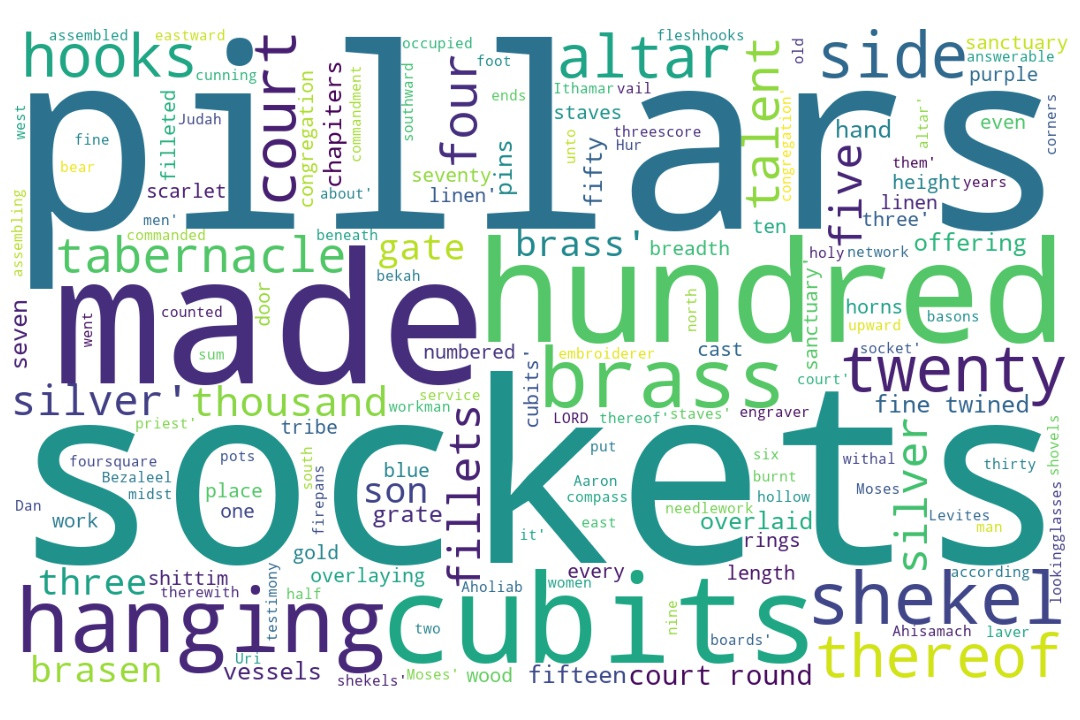
\includegraphics[width=\linewidth]{02OT-Exodus/Exodus38-WordCloud.jpg}
  \caption{Exodus 38 Word Cloud}
  \label{fig:Exodus 38 word Cloud}
\end{figure}


\marginpar{\scriptsize \centering \fcolorbox{bone}{lime}{\textbf{THE LAST PIECES}}\\ (Exodus 38:1--31) 
\begin{compactenum}[I.][8]
    \item A Place to \textbf{Burn} \index[scripture]{Exodus!Exo 38:01}(Exo 38:1)
    \item \textbf{Brass} Everywhere \index[scripture]{Exodus!Exo 38:02}\index[scripture]{Exodus!Exo 38:03}\index[scripture]{Exodus!Exo 38:05}\index[scripture]{Exodus!Exo 38:06}\index[scripture]{Exodus!Exo 38:08}\index[scripture]{Exodus!Exo 38:11}\index[scripture]{Exodus!Exo 38:17}\index[scripture]{Exodus!Exo 38:19}\index[scripture]{Exodus!Exo 38:20}\index[scripture]{Exodus!Exo 38:29}(Exo 38:2, 3, 5, 6, 8, 11, 17, 19, 20, 29)
    \item \textbf{Basons} \index[scripture]{Exodus!Exo 38:03}(Exo 38:3)  
    \item \textbf{Boards} \index[scripture]{Exodus!Exo 38:07}(Exo 38:7)  
    \item Somethings \textbf{Blue} \index[scripture]{Exodus!Exo 38:18}\index[scripture]{Exodus!Exo 38:23}(Exo 38:18, 23)  
    \item The \textbf{Book-keeping} \index[scripture]{Exodus!Exo 38:24--28}(Exo 38:24--28)  
\end{compactenum} }




\footnote{\textcolor[cmyk]{0.99998,1,0,0}{\hyperlink{TOC}{Return to end of Table of Contents.}}}\footnote{\href{https://audiobible.com/bible/exodus_38.html}{\textcolor[cmyk]{0.99998,1,0,0}{Exodus 38 Audio}}}\textcolor[cmyk]{0.99998,1,0,0}{And he made the \fcolorbox{bone}{lime}{altar of burnt offering} \emph{of} shittim wood: five cubits \emph{was} the length thereof, and five cubits the breadth thereof; \emph{it} \emph{was} foursquare; and three cubits the height thereof.}
[2] \textcolor[cmyk]{0.99998,1,0,0}{And he made the horns thereof on the four corners of it; the horns thereof were of the same: and he overlaid it with \fcolorbox{bone}{lime}{brass}.}
[3] \textcolor[cmyk]{0.99998,1,0,0}{And he made all the vessels of the altar, the pots, and the shovels, and the \fcolorbox{bone}{lime}{basons}, \emph{and} the fleshhooks, and the firepans: all the vessels thereof made he \emph{of} brass.}
[4] \textcolor[cmyk]{0.99998,1,0,0}{And he made for the altar a brasen grate of network under the compass thereof beneath unto the midst of it.}
[5] \textcolor[cmyk]{0.99998,1,0,0}{And he cast four rings for the four ends of the grate of brass, \emph{to} \emph{be} places for the staves.}
[6] \textcolor[cmyk]{0.99998,1,0,0}{And he made the staves \emph{of} shittim wood, and overlaid them with brass.}
[7] \textcolor[cmyk]{0.99998,1,0,0}{And he put the staves into the rings on the sides of the altar, to bear it withal; he made the altar hollow with \fcolorbox{bone}{lime}{boards}.}\\
\\
\P \textcolor[cmyk]{0.99998,1,0,0}{And he made the laver \emph{of} brass, and the foot of it \emph{of} brass, of the lookingglasses of \emph{the} \emph{women} assembling, which assembled \emph{at} the door of the tabernacle of the congregation.}\\
\\
\P \textcolor[cmyk]{0.99998,1,0,0}{And he made the court: on the south side southward the hangings of the court \fcolorbox{bone}{bone}{\emph{were}} \emph{of} fine twined linen, an hundred cubits:}
[10] \textcolor[cmyk]{0.99998,1,0,0}{Their \fcolorbox{bone}{bone}{pillars} \fcolorbox{bone}{bone}{\emph{were}} twenty, and their brasen \fcolorbox{bone}{bone}{sockets} twenty; the hooks of the \fcolorbox{bone}{bone}{pillars} and their fillets \fcolorbox{bone}{bone}{\emph{were}} \emph{of} silver.}
[11] \textcolor[cmyk]{0.99998,1,0,0}{And for the north side \emph{the} \emph{hangings} \fcolorbox{bone}{bone}{\emph{were}} an hundred cubits, their \fcolorbox{bone}{bone}{pillars} \fcolorbox{bone}{bone}{\emph{were}} twenty, and their \fcolorbox{bone}{bone}{sockets} of brass twenty; the hooks of the \fcolorbox{bone}{bone}{pillars} and their fillets \emph{of} silver.}
[12] \textcolor[cmyk]{0.99998,1,0,0}{And for the west side \fcolorbox{bone}{bone}{\emph{were}} hangings of fifty cubits, their \fcolorbox{bone}{bone}{pillars} ten, and their \fcolorbox{bone}{bone}{sockets} ten; the hooks of the \fcolorbox{bone}{bone}{pillars} and their fillets \emph{of} silver.}
[13] \textcolor[cmyk]{0.99998,1,0,0}{And for the east side eastward fifty cubits.}
[14] \textcolor[cmyk]{0.99998,1,0,0}{The hangings of the one side \emph{of} \emph{the} \emph{gate} \fcolorbox{bone}{bone}{\emph{were}} fifteen cubits; their \fcolorbox{bone}{bone}{pillars} three, and their \fcolorbox{bone}{bone}{sockets} three.}
[15] \textcolor[cmyk]{0.99998,1,0,0}{And for the other side of the court gate, on this hand and that hand, \fcolorbox{bone}{bone}{\emph{were}} hangings of fifteen cubits; their \fcolorbox{bone}{bone}{pillars} three, and their \fcolorbox{bone}{bone}{sockets} three.}
[16] \textcolor[cmyk]{0.99998,1,0,0}{All the hangings of the court round about \fcolorbox{bone}{bone}{\emph{were}} of fine twined linen.}
[17] \textcolor[cmyk]{0.99998,1,0,0}{And the \fcolorbox{bone}{bone}{sockets} for the \fcolorbox{bone}{bone}{pillars} \fcolorbox{bone}{bone}{\emph{were}} \emph{of} brass; the hooks of the \fcolorbox{bone}{bone}{pillars} and their fillets \emph{of} silver; and the overlaying of their chapiters \emph{of} silver; and all the \fcolorbox{bone}{bone}{pillars} of the court \fcolorbox{bone}{bone}{\emph{were}} filleted with silver.}
[18] \textcolor[cmyk]{0.99998,1,0,0}{And the hanging for the gate of the court \emph{was} needlework, \emph{of} \fcolorbox{bone}{lime}{blue}, and purple, and scarlet, and fine twined linen: and twenty cubits \emph{was} the length, and the height in the breadth \emph{was} five cubits, answerable to the hangings of the court.}
[19] \textcolor[cmyk]{0.99998,1,0,0}{And their \fcolorbox{bone}{bone}{pillars} \fcolorbox{bone}{bone}{\emph{were}} four, and their \fcolorbox{bone}{bone}{sockets} \emph{of} brass four; their hooks \emph{of} silver, and the overlaying of their chapiters and their fillets \emph{of} silver.}
[20] \textcolor[cmyk]{0.99998,1,0,0}{And all the pins of the tabernacle, and of the court round about, \fcolorbox{bone}{bone}{\emph{were}} \emph{of} brass.}\\
\\
\P \textcolor[cmyk]{0.99998,1,0,0}{This is the sum of the tabernacle, \emph{even} of the tabernacle of testimony, as it was counted, according to the commandment of Moses, \emph{for} the service of the Levites, by the hand of Ithamar, son to Aaron the priest.}
[22] \textcolor[cmyk]{0.99998,1,0,0}{And Bezaleel the son of Uri, the son of Hur, of the tribe of Judah, made all that the LORD commanded Moses.}
[23] \textcolor[cmyk]{0.99998,1,0,0}{And with him \emph{was} Aholiab, son of Ahisamach, of the tribe of Dan, an engraver, and a cunning workman, and an embroiderer in blue, and in purple, and in scarlet, and fine linen.}
[24] \textcolor[cmyk]{0.99998,1,0,0}{All the gold that was occupied for the work in all the work of the holy \emph{place}, even the gold of the offering, was twenty and nine talents, and seven hundred and thirty shekels, after the shekel of the sanctuary.}
[25] \textcolor[cmyk]{0.99998,1,0,0}{And the silver of them that were \fcolorbox{bone}{lime}{numbered} of the congregation \emph{was} an hundred talents, and a thousand seven hundred and threescore and fifteen shekels, after the shekel of the sanctuary:}
[26] \textcolor[cmyk]{0.99998,1,0,0}{A bekah for every man, \emph{that} \emph{is}, half a shekel, after the shekel of the sanctuary, for every one that went to be numbered, from twenty years old and upward, for six hundred thousand and three thousand and five hundred and fifty \emph{men}.}
[27] \textcolor[cmyk]{0.99998,1,0,0}{And of the hundred talents of silver were cast the \fcolorbox{bone}{bone}{sockets} of the sanctuary, and the \fcolorbox{bone}{bone}{sockets} of the vail; an hundred \fcolorbox{bone}{bone}{sockets} of the hundred talents, a talent for a socket.}
[28] \textcolor[cmyk]{0.99998,1,0,0}{And of the thousand seven hundred seventy and five shekels he made hooks for the \fcolorbox{bone}{bone}{pillars}, and overlaid their chapiters, and filleted them.}
[29] \textcolor[cmyk]{0.99998,1,0,0}{And the brass of the offering \emph{was} seventy talents, and two thousand and four hundred shekels.}
[30] \textcolor[cmyk]{0.99998,1,0,0}{And therewith he made the \fcolorbox{bone}{bone}{sockets} to the door of the tabernacle of the congregation, and the brasen altar, and the brasen grate for it, and all the vessels of the altar,}
[31] \textcolor[cmyk]{0.99998,1,0,0}{And the \fcolorbox{bone}{bone}{sockets} of the court round about, and the \fcolorbox{bone}{bone}{sockets} of the court gate, and all the pins of the tabernacle, and all the pins of the court round about.}

\chapter{Psalm 30}

\begin{figure}
  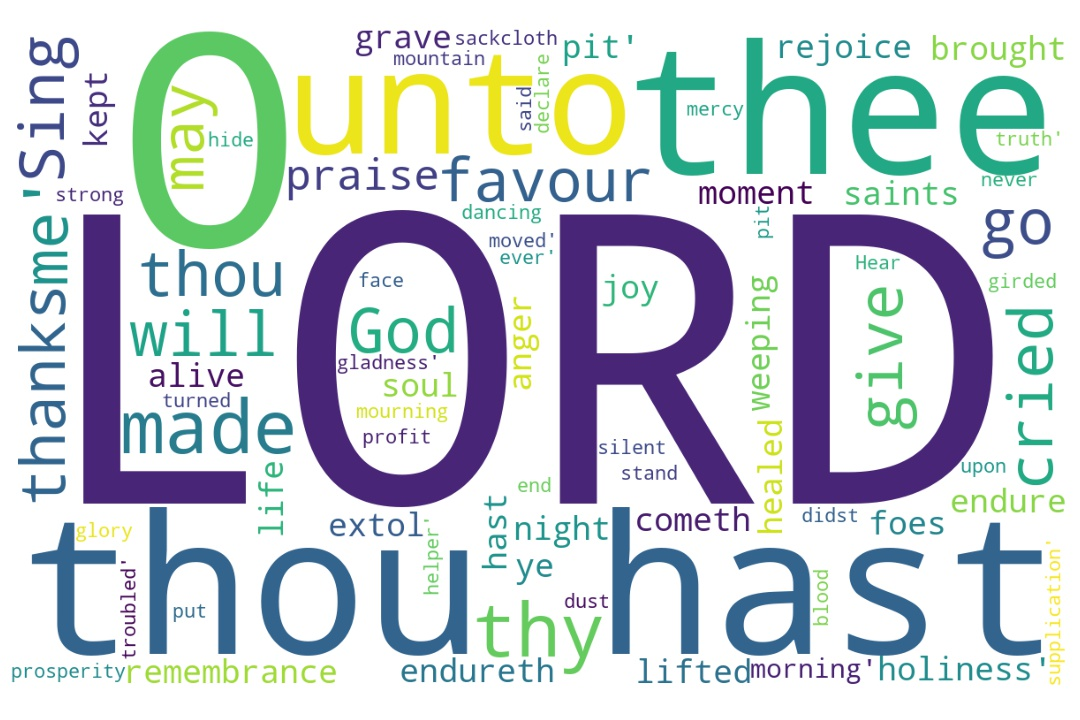
\includegraphics[width=\linewidth]{19OT-Psalms/Psalm30-WordCloud.jpg}
  \caption{Psalm 30 Word Cloud}
  \label{fig:Psalm 30 word Cloud}
\end{figure}


\marginpar{\scriptsize \centering \fcolorbox{bone}{lime}{\textbf{GOD'S FAVOUR}}\\ (Psalm 30:1--12) 
\begin{compactenum}[I.][8]
    \item David spared at the \textbf{Brink of Death} \index[scripture]{Psalms!Psa 030:03} (Psa 30:3)
    \item God's favor was David's \textbf{Basis for Deliverance} \index[scripture]{Psalms!Psa 030:05} (Psa 30:5)
    \item David's \textbf{Bad Declaration} \index[scripture]{Psalms!Psa 030:06} (Psa 30:6)
    \item David's \textbf{Better Decision}  \index[scripture]{Psalms!Psa 030:07} (Psa 30:7)
    \item David gets \textbf{Blessing instead of Dust} \index[scripture]{Psalms!Psa 030:09} (Psa 30:9)
    \item God changed David's \textbf{Bitterness into Dancing} \index[scripture]{Psalms!Psa 030:11} (Psa 30:11)
    \item David gets a \textbf{Bright Destiny} \index[scripture]{Psalms!Psa 030:12} (Psa 30:12)
\end{compactenum} }

%%%%%%%%%%%%%%%%%%%%%%%%%%%%%%%%%
%%%%%%%%%%%%%%%%%%%%%%%%%%%%%%%%%
\footnote{\textcolor[cmyk]{0.99998,1,0,0}{\hyperlink{TOC}{Return to end of Table of Contents.}}}\footnote{\href{https://www.audioverse.org/english/audiobibles/books/ENGKJV/O/Ps/1}{\textcolor[cmyk]{0.99998,1,0,0}{Psalms Audio}}}\textcolor[cmyk]{0.99998,1,0,0}{A Psalm \emph{and} Song \emph{at} the dedication of the house of David.}\\
\\
\textcolor[cmyk]{0.99998,1,0,0}{I will extol thee, O LORD; for thou hast lifted me up, and hast not made my foes to rejoice over me.}
[2] \textcolor[cmyk]{0.99998,1,0,0}{O LORD my God, I cried unto thee, and thou hast healed me.}
[3] \textcolor[cmyk]{0.99998,1,0,0}{O LORD, thou hast brought up my soul \fcolorbox{bone}{lime}{from the grave}: thou hast kept me alive, that I should not go down to the pit.}
[4] \textcolor[cmyk]{0.99998,1,0,0}{Sing unto the LORD, O ye saints of his, and give thanks at the remembrance of his holiness.}
[5] \textcolor[cmyk]{0.99998,1,0,0}{For his anger \emph{endureth} \emph{but} a moment; in \fcolorbox{bone}{lime}{his favour} \emph{is} life: weeping may endure for a night, but joy \emph{cometh} in the morning.}
[6] \textcolor[cmyk]{0.99998,1,0,0}{And in my prosperity I said, I shall \fcolorbox{bone}{lime}{never} be moved.}
[7] \textcolor[cmyk]{0.99998,1,0,0}{LORD, by \fcolorbox{bone}{lime}{thy favour} thou hast made my mountain to stand strong: thou didst hide thy face, \emph{and} I was troubled.}
[8] \textcolor[cmyk]{0.99998,1,0,0}{I \fcolorbox{bone}{lime}{cried to thee}, O LORD; and unto the LORD I made supplication.}
[9] \textcolor[cmyk]{0.99998,1,0,0}{What profit \emph{is} \emph{there} in my blood, when I go down to the pit? Shall the \fcolorbox{bone}{lime}{dust} praise thee? shall it declare thy truth?}
[10] \textcolor[cmyk]{0.99998,1,0,0}{Hear, O LORD, and have mercy upon me: LORD, be thou my helper.}
[11] \textcolor[cmyk]{0.99998,1,0,0}{Thou hast turned for me my mourning into \fcolorbox{bone}{lime}{dancing}: thou hast put off my sackcloth, and girded me with gladness;}
[12] \textcolor[cmyk]{0.99998,1,0,0}{To \fcolorbox{bone}{lime}{the end} that \emph{my} glory may sing praise to thee, and not be silent. O LORD my God, I will give thanks unto thee for ever.}

\chapter{Proverb 30}

\begin{figure}
  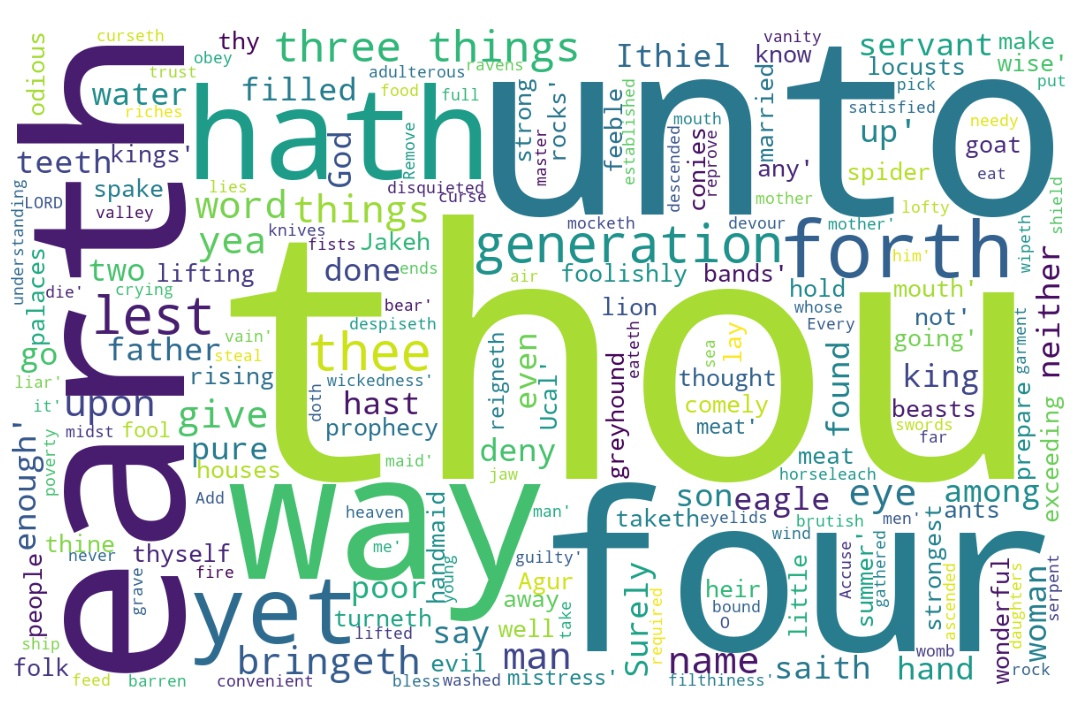
\includegraphics[width=\linewidth]{20OT-Proverbs/Proverb30-WordCloud.jpg}
  \caption{Proverb 30 Word Cloud}
  \label{fig:Proverb 30 word Cloud}
\end{figure}


\marginpar{\scriptsize \centering \fcolorbox{bone}{lime}{\textbf{A CONVERT TO WISDOM}}\\ (Proverb 30:1--33) 
\begin{compactenum}[I.][8]
    \item \textbf{Responds to Revealed Truth} \index[scripture]{Proverbs!Pro 30:01}(Pro 30:1)
    \item \textbf{Realizes his Brutish Condition} \index[scripture]{Proverbs!Pro 30:02-03}(Pro 30:2-3)
    \item \textbf{Respects God's Word} \index[scripture]{Proverbs!Pro 30:04-06}(Pro 30:4-6)
    \item \textbf{Requests Security from God} \index[scripture]{Proverbs!Pro 30:07-09}(Pro 30:7-9)
    \item Is \textbf{Repulsed by Wickedness} \index[scripture]{Proverbs!Pro 30:10-14}(Pro 30:10-14)
    \item \textbf{Recognizes Truth in Nature} \index[scripture]{Proverbs!Pro 30:15-31}(Pro 30:15-31)
    \item \textbf{Repents of Self-Promotion} \index[scripture]{Proverbs!Pro 30:32}(Pro 30:32)
\end{compactenum} }


\marginpar{\scriptsize \centering \fcolorbox{bone}{yellow}{\textbf{SEEING THE ASCENDANT ONE}}\\ (Proverb 30:1--33) 
\begin{compactenum}[I.][8]
    \item Who is \textbf{Listening} \index[scripture]{Proverbs!Pro 30:04}(Pro 30:4)
    \item Who is \textbf{Longing for Satisfaction} \index[scripture]{Proverbs!Pro 30:04}(Pro 30:4)
    \item Who is \textbf{Looking through Scripture} \index[scripture]{Proverbs!Pro 30:04}(Pro 30:4, \index[scripture]{Psalms!Psa 040:07}Psa 40:7)
    \item Who is \textbf{Laboring for Salvation} \index[scripture]{Proverbs!Pro 30:04}(Pro 30:4) -- only to find that he cannot succeed
    \item Who is \textbf{Lamenting Sin} \index[scripture]{Proverbs!Pro 30:04}(Pro 30:4) -- only to find that he cannot succeed
    \item Who is \textbf{Lost and Seeking} \index[scripture]{Proverbs!Pro 30:04}(Pro 30:4) 
    \item Who is \textbf{Lowly and Sorrowful} \index[scripture]{Proverbs!Pro 30:04}(Pro 30:4) 
\end{compactenum} }

\footnote{\textcolor[cmyk]{0.99998,1,0,0}{\hyperlink{TOC}{Return to end of Table of Contents.}}}\footnote{\href{https://www.audioverse.org/english/audiobibles/books/ENGKJV/O/Prov/1}{\textcolor[cmyk]{0.99998,1,0,0}{Proverbs Audio}}}\textcolor[cmyk]{0.99998,1,0,0}{The words of Agur the son of Jakeh, \emph{even} the \fcolorbox{bone}{lime}{prophecy}: the man spake unto Ithiel, even unto Ithiel and Ucal,}
[2] \textcolor[cmyk]{0.99998,1,0,0}{Surely I \emph{am} more \fcolorbox{bone}{lime}{brutish} than \emph{any} man, and have not the \fcolorbox{bone}{MYGOLD}{understanding} of a man.}\footnote{\textbf{Psalm 92:5-6} - O LORD, how great are thy works! and thy thoughts are very deep. [6] A brutish man knoweth not; neither doth a fool understand this.}
[3] \textcolor[cmyk]{0.99998,1,0,0}{I neither learned wisdom, nor have the knowledge of the holy.}
[4] \textcolor[cmyk]{0.99998,1,0,0}{Who hath ascended up into heaven, or descended? who hath gathered the wind in his fists? who hath bound the waters in a garment? who hath established all the ends of the earth? what \emph{is} his name, and what \emph{is} his son's name, if thou canst tell?}\footnote{\textbf{Exodus 3:13} - And Moses said unto God, Behold, when I come unto the children of Israel, and shall say unto them, The God of your fathers hath sent me unto you; and they shall say to me, What is his name? what shall I say unto them?}\footnote{\textbf{Job 26:8} - He bindeth up the waters in his thick clouds; and the cloud is not rent under them.}\footnote{\textbf{Job 38:37} - Who can number the clouds in wisdom? or who can stay the bottles of heaven,}\footnote{The connection is to the great KJV biblical truth of the Great Deep, starting back in Genesis.. The verse speaks to cosmology, or the structure of the universe. See ``garment'' in Hebrews 1:11 - They shall perish; but thou remainest; and they all shall wax old as doth a garment. See the typology pictured by the robe of a vindicated Mordecai in Esther 8:15 - And Mordecai went out from the presence of the king in royal apparel of blue and white, and with a great crown of gold, and with a garment of fine linen and purple: and the city of Shushan rejoiced and was glad. See the pure garment made of a single type of material in Deuteronomy 22:11 - Thou shalt not wear a garment of divers sorts, as of woollen and linen together. See the shepherd's garment in Jeremiah 43:12 - And I will kindle a fire in the houses of the gods of Egypt; and he shall burn them, and carry them away captives: and he shall array himself with the land of Egypt, as a shepherd putteth on his garment; and he shall go forth from thence in peace.  See the Lord's garment (the universe) described in Isaiah 50:9, 51:6, and 51:9.}
[5] \textcolor[cmyk]{0.99998,1,0,0}{Every \fcolorbox{bone}{lime}{word} of God \emph{is} pure: he \emph{is} a shield unto them that put their trust in him.}\footnote{\textbf{Psalm 12:6} - The words of the LORD are pure words: as silver tried in a furnace of earth, purified seven times.}
[6] \textcolor[cmyk]{0.99998,1,0,0}{Add thou not unto his words, lest he reprove thee, and thou be found a liar.}\footnote{\textbf{Revelation 22:18-19} -- For I testify unto every man that heareth the words of the prophecy of this book, If any man shall add unto these things, God shall add unto him the plagues that are written in this book: [19] And if any man shall take away from the words of the book of this prophecy, God shall take away his part out of the book of life, and out of the holy city, and from the things which are written in this book.}\footnote{\textbf{Deuteronomy 4:2} -- Ye shall not add unto the word which I command you, neither shall ye diminish ought from it, that ye may keep the commandments of the LORD your God which I command you.}
[7] \textcolor[cmyk]{0.99998,1,0,0}{Two \emph{things} have I \fcolorbox{bone}{lime}{required} of thee; deny me \emph{them} not before I die:}
[8] \textcolor[cmyk]{0.99998,1,0,0}{Remove far from me vanity and lies: give me neither poverty nor riches; feed me with food convenient for me:}
[9] \textcolor[cmyk]{0.99998,1,0,0}{Lest I be full, and deny \emph{thee}, and say, Who \emph{is} the LORD? or lest I be poor, and steal, and take the name of my God \emph{in} \emph{vain}.}
[10] \textcolor[cmyk]{0.99998,1,0,0}{Accuse not a servant unto his master, lest he curse thee, and thou be found guilty.}
[11] \textcolor[cmyk]{0.99998,1,0,0}{\emph{There} \emph{is} a generation \emph{that} curseth their father, and doth not bless their mother.}
[12] \textcolor[cmyk]{0.99998,1,0,0}{\fcolorbox{bone}{lime}{\emph{There} \emph{is} a generation} \emph{that} \emph{are} pure in their own eyes, and \emph{yet} is not washed from their filthiness.}
[13] \textcolor[cmyk]{0.99998,1,0,0}{\emph{There} \emph{is} a generation, O how lofty are their eyes! and their eyelids are lifted up.}
[14] \textcolor[cmyk]{0.99998,1,0,0}{\emph{There} \emph{is} a generation, whose teeth \emph{are} \emph{as} swords, and their jaw teeth \emph{as} knives, to devour the poor from off the earth, and the needy from \emph{among} men.}
[15] \textcolor[cmyk]{0.99998,1,0,0}{The \fcolorbox{bone}{lime}{horseleach} hath two daughters, \emph{crying}, Give, give. There are three \emph{things} \emph{that} are never satisfied, \emph{yea}, four \emph{things} say not, \emph{It} \emph{is} enough:}
[16] \textcolor[cmyk]{0.99998,1,0,0}{The grave; and the barren womb; the earth \emph{that} is not filled with water; and the fire \emph{that} saith not, \emph{It} \emph{is} enough.}
[17] \textcolor[cmyk]{0.99998,1,0,0}{The eye \emph{that} mocketh at \emph{his} father, and despiseth to obey \emph{his} mother, the ravens of the valley shall pick it out, and the young eagles shall eat it.}
[18] \textcolor[cmyk]{0.99998,1,0,0}{There be three \emph{things} \emph{which} are too wonderful for me, yea, four which I know not:}
[19] \textcolor[cmyk]{0.99998,1,0,0}{The way of an eagle in the air; the way of a serpent upon a rock; the way of a ship in the midst of the sea; and the way of a man with a maid.}
[20] \textcolor[cmyk]{0.99998,1,0,0}{Such \emph{is} the way of an adulterous woman; she eateth, and wipeth her mouth, and saith, I have done no wickedness.}
[21] \textcolor[cmyk]{0.99998,1,0,0}{For three \emph{things} the earth is disquieted, and for four \emph{which} it cannot bear:}
[22] \textcolor[cmyk]{0.99998,1,0,0}{For a servant when he reigneth; and a fool when he is filled with meat;}
[23] \textcolor[cmyk]{0.99998,1,0,0}{For an odious \emph{woman} when she is married; and an handmaid that is heir to her mistress.}
[24] \textcolor[cmyk]{0.99998,1,0,0}{There be four \emph{things} \emph{which} \emph{are} little upon the earth, but they \emph{are} exceeding wise:}
[25] \textcolor[cmyk]{0.99998,1,0,0}{The ants \emph{are} a people not strong, yet they prepare their meat in the summer;}
[26] \textcolor[cmyk]{0.99998,1,0,0}{The conies \emph{are} \emph{but} a feeble folk, yet make they their houses in the rocks;}
[27] \textcolor[cmyk]{0.99998,1,0,0}{The locusts have no king, yet go they forth all of them by bands;}
[28] \textcolor[cmyk]{0.99998,1,0,0}{The spider taketh hold with her hands, and is in kings' palaces.}
[29] \textcolor[cmyk]{0.99998,1,0,0}{There be three \emph{things} which go well, yea, four are comely in going:}
[30] \textcolor[cmyk]{0.99998,1,0,0}{A lion \emph{which} \emph{is} strongest among beasts, and turneth not away for any;}
[31] \textcolor[cmyk]{0.99998,1,0,0}{A greyhound; an he goat also; and a king, against whom \emph{there} \emph{is} no rising up.}
[32] \textcolor[cmyk]{0.99998,1,0,0}{If thou hast done foolishly in \fcolorbox{bone}{lime}{lifting up thyself}, or if thou hast thought evil, \emph{lay} thine hand upon thy mouth.}
[33] \textcolor[cmyk]{0.99998,1,0,0}{Surely the churning of milk bringeth forth butter, and the wringing of the nose bringeth forth blood: so the forcing of wrath bringeth forth strife.}



\end{document}


